\documentclass[11pt,a4paper]{article}

\usepackage{times}
\usepackage{url}
\usepackage{graphicx}

\pagestyle{empty}

\textheight=25cm
\textwidth=15cm
\topmargin=-2cm
\oddsidemargin=0cm

\begin{document}

\begin{center}
  Ole Nielsen \\
  Computational Scientist \\
  Australia-Indonesia Facility for Disaster Reduction, AusAID Jakarta \\
  P: +62 811 820 4637,\ \ \ E: Ole.Nielsen@aifdr.org
\end{center}
\begin{center}
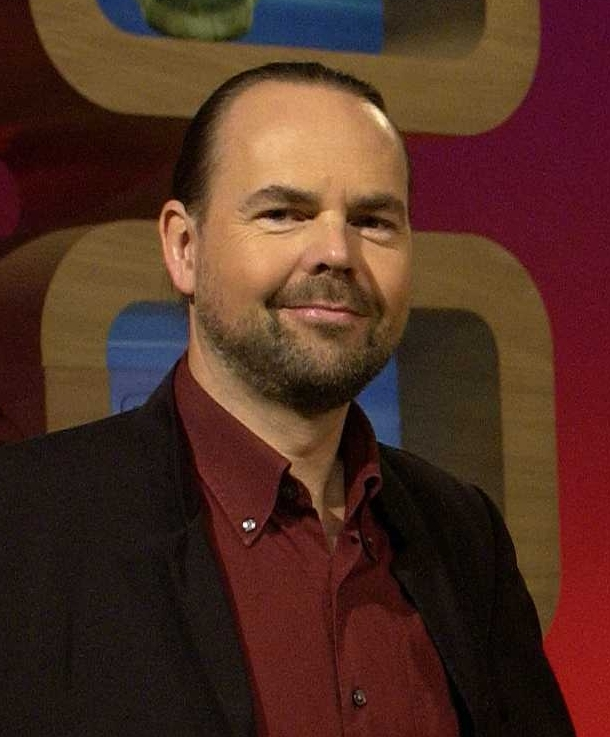
\includegraphics[width=60mm,keepaspectratio=true]{ole.jpg}
\end{center}


\begin{center}
  \hrulefill \\
  {\bf Mission} \\[-0.2cm]
  \hrulefill
\end{center}
\emph{Applying science and technology to problems that matter.}
\begin{center}
  \hrulefill \\
  {\bf Biography} \\[-0.2cm]
  \hrulefill
\end{center}


Ole Nielsen has been an Open Source adopter, promotor and developer
since the early nineties during his career as technical consultant,
academic researcher, government scientist and development
professional within an aid organisation.

Ole has a double Master's degree in Mathematics and Computer Science
as well as a PhD in scientific computing from universities in Denmark.
After a short stint as a consultant in parallel computing, he joined
the Australian National University researching wavelet techniques for
predictive modelling, large scale data mining and bio-informatics. Ole
took up a position as a computational scientist at Geoscience
Australia in 2003 where he was responsible for the development of a
hydrodynamic modelling capability and its applications in tsunami
impact modelling for Australian emergency management agencies. This
work was awarded the Emergency Management Australia "Safer Communities
Award" in 2005 and 2007 as well as the "Asia-Pacific Spatial
Excellence Award" in 2007. Ole joined AusAID in
Jakarta in 2010 to support the Indonesian government in multi-hazard disaster
risk reduction.

Ole is the lead developer of the Open Source packages ANUGA
(hydrodynamc fluid mechanics) --- which was featured on Australian TV
(The New Inventors) in June 2009 --- Risiko (Spatial modelling of impact from natural disasters) and PyPar (Parallel computing for
Python) as well as a number of smaller scientific toolkits. Ole has chosen Python for most of these because of it is the best tool for scientific computing.

Ole is a
dedicated advocate for adherence to regression testing, revision
control, good error messages and agile approaches to ensure software quality

Ole has been instrumental in elevating the awareness of Open Source
in government organisations by demonstrating the strategic advantage
of publicising tools as Open Source, promoting Linux and Python as the
platform of choice for scientific computing, building Beowulf clusters
and participating in a tender panel for a government wide survey of
the uptake and use of Open Source.


\end{document}

